
\documentclass[letterpaper,hide notes,xcolor={table,svgnames},pdftex]{beamer}
\def\showexamples{t}


%\usepackage[svgnames]{xcolor}

%% Demo talk
%\documentclass[letterpaper,notes=show]{beamer}

\usecolortheme{crane}
\setbeamertemplate{navigation symbols}{}

\usetheme{MyPittsburgh}
%\usetheme{Frankfurt}

%\usepackage{tipa}

\usepackage{hyperref}
\usepackage{graphicx,xspace}
\usepackage[normalem]{ulem}

\newcommand\SF[1]{$\bigstar$\footnote{SF: #1}}



\newcounter{tmpnumSlide}
\newcounter{tmpnumNote}

% old question code
%\newcommand\question[1]{{$\bigstar$ \small \onlySlide{2}{#1}}}
% \newcommand\nquestion[1]{\ifdefined \presentationonly \textcircled{?} \fi \note{\par{\Large \textbf{?}} #1}}
% \newcommand\nanswer[1]{\note{\par{\Large \textbf{A}} #1}}


 \newcommand\mnote[1]{%
   \addtocounter{tmpnumSlide}{1}
   \ifdefined\showcues {~\tiny\fbox{\arabic{tmpnumSlide}}}\fi
   \note{\setlength{\parskip}{1ex}\addtocounter{tmpnumNote}{1}\textbf{\Large \arabic{tmpnumNote}:} {#1\par}}}

\newcommand\mmnote[1]{\note{\setlength{\parskip}{1ex}#1\par}}

%\newcommand\mnote[2][]{\ifdefined\handoutwithnotes {~\tiny\fbox{#1}}\fi
% \note{\setlength{\parskip}{1ex}\textbf{\Large #1:} #2\par}}

%\newcommand\mnote[2][]{{\tiny\fbox{#1}} \note{\setlength{\parskip}{1ex}\textbf{\Large #1:} #2\par}}

\newcommand\mquestion[2]{{~\color{red}\fbox{?}}\note{\setlength{\parskip}{1ex}\par{\Large \textbf{?}} #1} \note{\setlength{\parskip}{1ex}\par{\Large \textbf{A}} #2\par}\ifdefined \presentationonly \pause \fi}

\newcommand\blackboard[1]{%
\ifdefined   \showblackboard
  {#1}
  \else {\begin{center} \fbox{\colorbox{blue!30}{%
         \begin{minipage}{.95\linewidth}%
           \hspace{\stretch{1}} Some space intentionally left blank; done at the blackboard.%
         \end{minipage}}}\end{center}}%
         \fi%
}



%\newcommand\q{\tikz \node[thick,color=black,shape=circle]{?};}
%\newcommand\q{\ifdefined \presentationonly \textcircled{?} \fi}

\usepackage{listings}
\lstset{%
  keywordstyle=\bfseries,
  aboveskip=15pt,
  belowskip=15pt,
  captionpos=b,
  identifierstyle=\ttfamily,
  escapeinside={(*@}{@*)},
  stringstyle=\ttfamiliy,
  frame=lines,
  numbers=left, basicstyle=\scriptsize, numberstyle=\tiny, stepnumber=0, numbersep=2pt}

\usepackage{siunitx}
\newcommand\sius[1]{\num[group-separator = {,}]{#1}\si{\micro\second}}
\newcommand\sims[1]{\num[group-separator = {,}]{#1}\si{\milli\second}}
\newcommand\sins[1]{\num[group-separator = {,}]{#1}\si{\nano\second}}
\sisetup{group-separator = {,}, group-digits = true}

%% -------------------- tikz --------------------
\usepackage{tikz}
\usetikzlibrary{positioning}
\usetikzlibrary{arrows,backgrounds,automata,decorations.shapes,decorations.pathmorphing,decorations.markings,decorations.text}

\tikzstyle{place}=[circle,draw=blue!50,fill=blue!20,thick, inner sep=0pt,minimum size=6mm]
\tikzstyle{transition}=[rectangle,draw=black!50,fill=black!20,thick, inner sep=0pt,minimum size=4mm]

\tikzstyle{block}=[rectangle,draw=black, thick, inner sep=5pt]
\tikzstyle{bullet}=[circle,draw=black, fill=black, thin, inner sep=2pt]

\tikzstyle{pre}=[<-,shorten <=1pt,>=stealth',semithick]
\tikzstyle{post}=[->,shorten >=1pt,>=stealth',semithick]
\tikzstyle{bi}=[<->,shorten >=1pt,shorten <=1pt, >=stealth',semithick]

\tikzstyle{mut}=[-,>=stealth',semithick]

\tikzstyle{treereset}=[dashed,->, shorten >=1pt,>=stealth',thin]

\usepackage{ifmtarg}
\usepackage{xifthen}
\makeatletter
% new counter to now which frame it is within the sequence
\newcounter{multiframecounter}
% initialize buffer for previously used frame title
\gdef\lastframetitle{\textit{undefined}}
% new environment for a multi-frame
\newenvironment{multiframe}[1][]{%
\ifthenelse{\isempty{#1}}{%
% if no frame title was set via optional parameter,
% only increase sequence counter by 1
\addtocounter{multiframecounter}{1}%
}{%
% new frame title has been provided, thus
% reset sequence counter to 1 and buffer frame title for later use
\setcounter{multiframecounter}{1}%
\gdef\lastframetitle{#1}%
}%
% start conventional frame environment and
% automatically set frame title followed by sequence counter
\begin{frame}%
\frametitle{\lastframetitle~{\normalfont(\arabic{multiframecounter})}}%
}{%
\end{frame}%
}
\makeatother

\makeatletter
\newdimen\tu@tmpa%
\newdimen\ydiffl%
\newdimen\xdiffl%
\newcommand\ydiff[2]{%
    \coordinate (tmpnamea) at (#1);%
    \coordinate (tmpnameb) at (#2);%
    \pgfextracty{\tu@tmpa}{\pgfpointanchor{tmpnamea}{center}}%
    \pgfextracty{\ydiffl}{\pgfpointanchor{tmpnameb}{center}}%
    \advance\ydiffl by -\tu@tmpa%
}
\newcommand\xdiff[2]{%
    \coordinate (tmpnamea) at (#1);%
    \coordinate (tmpnameb) at (#2);%
    \pgfextractx{\tu@tmpa}{\pgfpointanchor{tmpnamea}{center}}%
    \pgfextractx{\xdiffl}{\pgfpointanchor{tmpnameb}{center}}%
    \advance\xdiffl by -\tu@tmpa%
}
\makeatother
\newcommand{\copyrightbox}[3][r]{%
\begin{tikzpicture}%
\node[inner sep=0pt,minimum size=2em](ciimage){#2};
\usefont{OT1}{phv}{n}{n}\fontsize{4}{4}\selectfont
\ydiff{ciimage.south}{ciimage.north}
\xdiff{ciimage.west}{ciimage.east}
\ifthenelse{\equal{#1}{r}}{%
\node[inner sep=0pt,right=1ex of ciimage.south east,anchor=north west,rotate=90]%
{\raggedleft\color{black!50}\parbox{\the\ydiffl}{\raggedright{}#3}};%
}{%
\ifthenelse{\equal{#1}{l}}{%
\node[inner sep=0pt,right=1ex of ciimage.south west,anchor=south west,rotate=90]%
{\raggedleft\color{black!50}\parbox{\the\ydiffl}{\raggedright{}#3}};%
}{%
\node[inner sep=0pt,below=1ex of ciimage.south west,anchor=north west]%
{\raggedleft\color{black!50}\parbox{\the\xdiffl}{\raggedright{}#3}};%
}
}
\end{tikzpicture}
}


%% --------------------

%\usepackage[excludeor]{everyhook}
%\PushPreHook{par}{\setbox0=\lastbox\llap{MUH}}\box0}

%\vspace*{\stretch{1}

%\setbox0=\lastbox \llap{\textbullet\enskip}\box0}

\setlength{\parskip}{\fill}

\newcommand\noskips{\setlength{\parskip}{1ex}}
\newcommand\doskips{\setlength{\parskip}{\fill}}

\newcommand\xx{\par\vspace*{\stretch{1}}\par}
\newcommand\xxs{\par\vspace*{2ex}\par}
\newcommand\tuple[1]{\langle #1 \rangle}
\newcommand\code[1]{{\sf \footnotesize #1}}
\newcommand\ex[1]{\uline{Example:} \ifdefined \presentationonly \pause \fi
  \ifdefined\showexamples#1\xspace\else{\uline{\hspace*{2cm}}}\fi}

\newcommand\ceil[1]{\lceil #1 \rceil}


\AtBeginSection[]
{
   \begin{frame}
       \frametitle{Outline}
       \tableofcontents[currentsection]
   \end{frame}
}



\pgfdeclarelayer{edgelayer}
\pgfdeclarelayer{nodelayer}
\pgfsetlayers{edgelayer,nodelayer,main}

\tikzstyle{none}=[inner sep=0pt]
\tikzstyle{rn}=[circle,fill=Red,draw=Black,line width=0.8 pt]
\tikzstyle{gn}=[circle,fill=Lime,draw=Black,line width=0.8 pt]
\tikzstyle{yn}=[circle,fill=Yellow,draw=Black,line width=0.8 pt]
\tikzstyle{empty}=[circle,fill=White,draw=Black]
\tikzstyle{bw} = [rectangle, draw, fill=blue!20, 
    text width=4em, text centered, rounded corners, minimum height=2em]
    
    \newcommand{\CcNote}[1]{% longname
	This work is licensed under the \textit{Creative Commons #1 3.0 License}.%
}
\newcommand{\CcImageBy}[1]{%
	\includegraphics[scale=#1]{creative_commons/cc_by_30.pdf}%
}
\newcommand{\CcImageSa}[1]{%
	\includegraphics[scale=#1]{creative_commons/cc_sa_30.pdf}%
}
\newcommand{\CcImageNc}[1]{%
	\includegraphics[scale=#1]{creative_commons/cc_nc_30.pdf}%
}
\newcommand{\CcGroupBySa}[2]{% zoom, gap
	\CcImageBy{#1}\hspace*{#2}\CcImageNc{#1}\hspace*{#2}\CcImageSa{#1}%
}
\newcommand{\CcLongnameByNcSa}{Attribution-NonCommercial-ShareAlike}

\newenvironment{changemargin}[1]{% 
  \begin{list}{}{% 
    \setlength{\topsep}{0pt}% 
    \setlength{\leftmargin}{#1}% 
    \setlength{\rightmargin}{1em}
    \setlength{\listparindent}{\parindent}% 
    \setlength{\itemindent}{\parindent}% 
    \setlength{\parsep}{\parskip}% 
  }% 
  \item[]}{\end{list}} 



\usepackage{tikz-3dplot}

\title{Lecture 26 --- Refactoring}

\author{Jeff Zarnett \& Patrick Lam \\ \small \texttt{jzarnett@uwaterloo.ca} \&\texttt{p.lam@ece.uwaterloo.ca}}
\institute{Department of Electrical and Computer Engineering \\[-1ex]
  University of Waterloo}
\date{\today}

\begin{document}

\begin{frame}
  \titlepage
\end{frame}


\begin{frame}
\frametitle{Refactoring}
\begin{changemargin}{1cm}

We have mentioned refactoring very frequently in the course.

\alert{Refactoring} incrementally improves code quality using local, semantics-preserving changes to the code.

\end{changemargin}
\end{frame}

\begin{frame}
\frametitle{Refactoring}
\begin{changemargin}{1cm}

More restrictive definition: refactoring must make code clearer.

Ease of understanding is not our only goal, so we will use the more inclusive definition.

Constrast this against a performance optimization: makes code harder to understand, but faster.

\end{changemargin}
\end{frame}


\begin{frame}
\frametitle{Refactoring}
\begin{changemargin}{1cm}

Two small clarifications:

\begin{itemize}
\item {\bf Local}: Refactoring should not affect unrelated parts of the
program. \mnote{it should only change the parts of the program that you're 
refactoring. When you commit a refactoring to the repository,
you should be sure to only commit the source files that got refactored.}
\item {\bf Semantics-preserving}: The behaviour
of the refactored code should be identical to the behaviour of the
original code. \mnote{If some tool did the refactoring, you can usually be sure
that it was semantics-preserving. Otherwise, your unit tests will help
ensure that you didn't change anything.}
\end{itemize}

\end{changemargin}
\end{frame}


\begin{frame}
\frametitle{Why Refactor?}
\begin{changemargin}{1cm}

\begin{itemize}
	\item Change the design\\
	 \quad(Nobody gets it 100\% right on the first try).
	\item Maintain good structure \& prevent decay.
	\item Make code easier to change.
	\item Prevent future errors.
	\item Make it easy to understand.
\end{itemize}

\end{changemargin}
\end{frame}

\begin{frame}
\frametitle{Types of Refactoring}
\begin{changemargin}{1cm}
\begin{itemize}
	\item Composing methods
	\item Moving features between objects
	\item Organizing data
	\item Simplifying conditionals
	\item Making method calls simpler
	\item Generalizations
\end{itemize}

\end{changemargin}
\end{frame}


\begin{frame}
\frametitle{Refactoring Process}
\begin{changemargin}{1cm}

\begin{enumerate}
	\item Create unit tests (if needed)
	\item Run unit tests
	\item Make changes
	\item Re-run unit tests
	\item Evaluate results
\end{enumerate}

Hopefully, you already have unit tests so you can skip step 1. If not - why not?

\end{changemargin}
\end{frame}



\begin{frame}[fragile]
\frametitle{Refactoring Example: Extract Method}
\begin{changemargin}{1cm}

\begin{verbatim}
// (1) make sure the code only runs on mac os x
boolean mrjVersionExists = 
     System.getProperty(``mrj.version'') != null;
boolean osNameExists = 
     System.getProperty(``os.name'')
           .startsWith(``Mac OS'');

if ( !mrjVersionExists || !osNameExists) {
  System.err.println(
       ``Not running on a Mac OS X system.'');
  System.exit(1);
}
\end{verbatim}
\end{changemargin}
\end{frame}

\begin{frame}[fragile]
\frametitle{Refactoring Example: Extract Method}
\begin{changemargin}{1cm}

\begin{verbatim}
// (2, 3) do all the preferences stuff
// and get the default color
preferences = Preferences
          .userNodeForPackage(this.getClass());
int r = preferences.getInt(CURTAIN_R, 0);
int g = preferences.getInt(CURTAIN_G, 0);
int b = preferences.getInt(CURTAIN_B, 0);
int a = preferences.getInt(CURTAIN_A, 255);
currentColor = new Color(r,g,b,a);
\end{verbatim}



\end{changemargin}
\end{frame}


\begin{frame}[fragile]
\frametitle{Refactoring Example: Extract Method}
\begin{changemargin}{1cm}

We can instead split this into three sub-methods.

\begin{verbatim}

  dieIfNotRunningOnMacOsX();
  connectToPreferences();
  getDefaultColor();


\end{verbatim}
\end{changemargin}
\end{frame}

\begin{frame}
\frametitle{Refactoring: Extract Method}
\begin{changemargin}{1cm}

This is useful when the code does the same thing many times.

Replace all the clones with a call to a single method.

Update the code once to update all.

\end{changemargin}
\end{frame}

\begin{frame}
\frametitle{Refactoring: Extract Method}
\begin{changemargin}{1cm}

Methods should do one conceptual thing.

A good test: can you come up with a name for it?

We are putting more design into the code.

Eclipse supports doing this in one click.

\end{changemargin}
\end{frame}

\begin{frame}[fragile]
\frametitle{Refactoring: Replace Magic Number}
\begin{changemargin}{1cm}
 Using symbolic constants is often better coding practice
than putting numbers directly into the code.

\begin{verbatim}
double potentialEnergy(double mass, double height) {
     return mass * height * 9.81;
}
\end{verbatim}

\end{changemargin}
\end{frame}

\begin{frame}[fragile]
\frametitle{Refactoring: Replace Magic Number}
\begin{changemargin}{1cm}
 Using symbolic constants is often better coding practice
than putting numbers directly into the code.

\begin{verbatim}
static final double GRAVITATIONAL_CONSTANT = 9.81;

double potentialEnergy(double mass, double height) {
     return mass * GRAVITATIONAL_CONSTANT * height;
}
\end{verbatim}

Easier to understand and easier to update.

\end{changemargin}
\end{frame}

\begin{frame}[fragile]
\frametitle{Refactoring: Rename Variable}
\begin{changemargin}{1cm}
One minor example of refactoring is renaming a variable.


\begin{verbatim}
DateTime creationTime;

public DateTime getCreationTime(){
    return creationTime;
}

public void setCreationTime(DateTime newTime) {
    this.creationTime = newCreationTime;
}

\end{verbatim}

We change the variable and methods for more clarity.

\end{changemargin}
\end{frame}

\begin{frame}[fragile]
\frametitle{Refactoring: Rename Variable}
\begin{changemargin}{1cm}
One minor example of refactoring is renaming a variable.


\begin{verbatim}
DateTime creationDateTime;

public DateTime getCreationDateTime(){
    return creationDateTime;
}

public void setCreationDateTime(DateTime newDateTime) {
    this.creationDateTime = newCreationDateTime;
}

\end{verbatim}

We change the variable and methods for more clarity.

\end{changemargin}
\end{frame}


\begin{frame}
\frametitle{Refactoring: Limitations}
\begin{changemargin}{1cm}

Diminishing returns as more is changed.

Changing interfaces might not be possible.

External systems (e.g., database) might constrain changes.

\end{changemargin}
\end{frame}

\begin{frame}
\frametitle{Refactoring vs Performance}
\begin{changemargin}{1cm}

Refactoring aims to improve \emph{non-functional properties} of the code; performance may get better, worse, or stay the same.

Our goal is easier to maintain code.

Example: split one loop into two separate loops.

\end{changemargin}
\end{frame}

\begin{frame}
\frametitle{When to Refactor}
\begin{changemargin}{1cm}

\begin{itemize}
	\item Continuously?\mnote{Refactoring done continuously helps prevent the ``pile of dirty dishes'' problem, but it can lead to spending too much time tinkering with the refactoring and not implementing the code.}
	\item Fixed Schedule?\mnote{If we refactor on a fixed schedule, say, every three months, that allows us to take some time and examine the code and do a lot of refactorings all at once.}
	\item When Fixing a Bug?\mnote{Some advocate for making changes while we fix bugs: if we notice something when we're re-examining code, we fix it right away. However, this strategy is dangerous because it conflates the bug fix with the structural change. }
	\item At the End of a Project?\mnote{In other cases, it's desirable to refactor once the code for a project is complete (before it goes into maintenance mode). }
	\item At the Start of a Project?\mnote{Lastly, we might consider refactoring at the start of a project; before we open up the module and begin to make our changes and additions, we clean up the code and then begin the new project.}
\end{itemize}

\end{changemargin}
\end{frame}

\begin{frame}
\frametitle{List of Refactorings}
\begin{changemargin}{1cm}

\mnote{These refactorings are organized differently than last lecture.}


Techniques that allow for more abstraction:
\begin{itemize}
\item \emph{Encapsulate Field}: force code to access the field with getter and setter methods.
\item \emph{Generalize Type}: create more general types to allow for more code sharing.
\item \emph{Replace conditional with polymorphism}: use inheritance and virtual dispatch instead of a conditional.
\end{itemize}


\end{changemargin}
\end{frame}

\begin{frame}
\frametitle{List of Refactorings}
\begin{changemargin}{1cm}

Techniques for breaking code apart into more logical pieces:
\begin{itemize}
\item \emph{Extract Method}: as seen above, pull out part of a larger method into a new method.
\item \emph{Extract Class}: moves code from an existing class into a new class.
\end{itemize}

\end{changemargin}
\end{frame}


\begin{frame}
\frametitle{List of Refactorings}
\begin{changemargin}{1cm}
Techniques for integrating code that's needlessly spread apart:
\begin{itemize}
\item \emph{Inline Method}: integrate a copy of the body of a method into its calling method.
\item \emph{Inline Class}: put all of the fields and methods of a class into another class and erase the original.
\end{itemize}

\end{changemargin}
\end{frame}


\begin{frame}
\frametitle{List of Refactorings}
\begin{changemargin}{1cm}

Techniques for improving names and location of code:
\begin{itemize}
\item \emph{Move Method/Field}: move to a more appropriate class or source file.
\item \emph{Rename Method/Field}: changing the name into a new one that better reveals its purpose.
\item \emph{Pull Up}: in OOP, move to a superclass.
\item \emph{Push Down}: in OOP, move to a subclass.
\end{itemize}


\end{changemargin}
\end{frame}


\begin{frame}
\frametitle{Antipatterns}
\begin{changemargin}{1cm}

Antipatterns are like antimatter -- the opposite of how software should be designed.

In software, a way of coding that makes errors more likely.

Not only for software (e.g., management antipatterns).

\end{changemargin}
\end{frame}

\begin{frame}
\frametitle{The Antipatterns Family}
\begin{changemargin}{1cm}

Some common antipatterns you might encounter:

\begin{itemize}
	\item The Blob
	\item Lava Flow
	\item Functional Decomposition
	\item Copy-and-Paste Programming
	\item Poltergeists
	\item Golden Hammer
	\item Exceptions as Control Flow
	\item Spaghetti Code
\end{itemize}


\end{changemargin}
\end{frame}


\begin{frame}
\frametitle{Antipatterns: The Blob}
\begin{changemargin}{1cm}
One object does basically everything.

From the horror movie: the blob just keeps growing.

Too much code/logic centralized in this one class.

Solution: extract methods and classes so it is spread out.


\end{changemargin}
\end{frame}

\begin{frame}
\frametitle{Antipatterns: Lava Flow}
\begin{changemargin}{1cm}
Old dead (useless) code hanging around in the software.

Nobody changes/deletes it for fear of breaking something.

From the geological phenomenon: lava flows then solidifies.

Time wasted testing and refactoring this dead code.

Solution: delete it (restore from version control if needed).

\end{changemargin}
\end{frame}

\begin{frame}
\frametitle{Antipatterns: Functional Decomposition}
\begin{changemargin}{1cm}
Code resembles a structural language when using OOP.

Often caused by non-OOP programmers writing in Java/C\#.

Solution: Extract classes and methods, pull up common code.

\end{changemargin}
\end{frame}

\begin{frame}
\frametitle{Antipatterns: Copy-and-Paste Programming}
\begin{changemargin}{1cm}
Code is copy-and-pasted; possibly modified slightly each time.

Copies can be slightly different so bugs will not be solved if one is updated and the rest are not.

Solution: extract class or method to replace all these copies.

\end{changemargin}
\end{frame}

\begin{frame}
\frametitle{Antipatterns: Poltergeists}
\begin{changemargin}{1cm}
Poltergeist (English): a ghost that allegedly causes noise or destruction and then vanishes.

Poltergeists: classes with limited roles and effective life cycles.

Objects that pop in, do one thing, then vanish.

Waste of resources and inefficient.

Solution: Call the Ghostbusters!\\
\quad\quad Actually, inline their functionality to other classes.


\end{changemargin}
\end{frame}

\begin{frame}
\frametitle{Antipatterns: Golden Hammer}
\begin{changemargin}{1cm}
``When all you have is hammer, everything looks like a nail.''

Familiar concept or architecture applied to everything, whether that makes sense or not.

Solution: Refactor the code to more appropriate design.

\end{changemargin}
\end{frame}

\begin{frame}
\frametitle{Antipatterns: Exceptions as Control Flow}
\begin{changemargin}{1cm}
``That error is supposed to happen.''

Exceptions should not be considered normal.

Exceptions are expensive to generate and handle.

Solution: Refactor to avoid Exceptions where they are expected.

\end{changemargin}
\end{frame}


\begin{frame}
\frametitle{Antipatterns: Spaghetti Code}
\begin{changemargin}{1cm}
Program with little or no structure.

Typically small number of objects with long methods.

No structure means difficult to extend or change things.

Solution: refactor until the code has appropriate structure.


\end{changemargin}
\end{frame}

\begin{frame}
\frametitle{Refactoring: Examples}
\begin{changemargin}{1cm}

We'll continue by talking about the
refactorings in more detail; perhaps this will help you understand the
goals of refactoring, so that you can do it in your own code.

\end{changemargin}
\end{frame}


\begin{frame}
\frametitle{Refactoring: Encapsulate Field}
\begin{changemargin}{1cm}

Java programming practice: private fields, public accessor methods. 

Replace {\tt x.foo} with {\tt x.getFoo()} and {\tt x.setFoo(y)}. 

Why? Modularity, logging, flexibility, etc. \mnote{One implication is that you can change the way you store the internal
data inside a class, and it won't affect any other classes. For instance,
you can have a {\tt Point} class which you initially implement using 
x/y coordinates, and then transparently change it to using polar
coordinates without having to change any of the users of the {\tt Point}.}

Should all fields be encapsulated? \mnote{For instance, if you 
have a class which represents an RGB colour, it's probably OK to have 
public fields for the red, green and blue fields.}

\end{changemargin}
\end{frame}

\begin{frame}
\frametitle{Refactoring: Pull Up Method}
\begin{changemargin}{1cm}

This refactoring is an example of a generalization.

\begin{center}
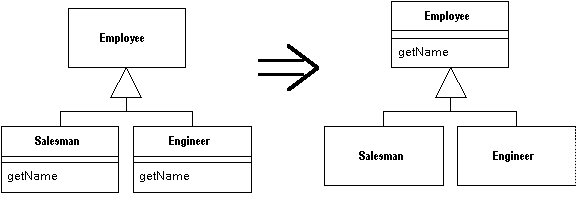
\includegraphics[width=0.85\textwidth]{images/pullUpMethod.png}
\end{center}

\mnote{What we can see here is that the two subclasses {\tt Salesman} and
{\tt Engineer} both have a common method {\tt getName}, with
identical behaviour. It makes sense to move the method to the common
superclass {\tt Employee}.}

\end{changemargin}
\end{frame}


\begin{frame}
\frametitle{Refactoring: Push Down Method}
\begin{changemargin}{1cm}

Sometimes we want to do the opposite.

\begin{center}
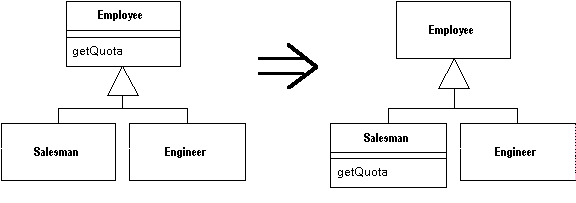
\includegraphics[width=0.85\textwidth]{images/pushDownMethod.png}
\end{center}


\mnote{In this case, the original design was flawed: {\tt Engineer}s don't
have quotas, only {\tt Salesman}. So we improve the design by 
putting {\tt getQuota} where it should be.}

\mnote{I didn't show you the code, only the UML, but the transformation to the
code should be obvious. Note that in both cases, it's not supposed
to change the behaviour of the program, only improve its design.}

\end{changemargin}
\end{frame}

\begin{frame}
\frametitle{Refactoring: Inline Class}
\begin{changemargin}{1cm}

Here, we get rid of helper classes that aren't useful.

\begin{center}
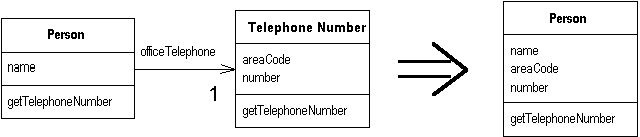
\includegraphics[width=0.85\textwidth]{images/inlineClass.png}
\end{center}



\mnote{The UML transformation corresponds to a code transformation where we
fold the {\tt areaCode} and {\tt number} fields, along with the
{\tt getTelephoneNumber} method, into the containing {\tt Person} class.
Maybe we found that no one else was using the {\tt Telephone Number} class.
Be sure to delete the class after you've inlined it.}

\end{changemargin}
\end{frame}

\begin{frame}[fragile]
\frametitle{Fixing an Antipattern: Exception as Control Flow}
\begin{changemargin}{1cm}

In this example, we are (ab)using an Exception and handler:

\begin{lstlisting}[language={Java}]
try {
   fileReader.readFile(
      fileSelector.getSelection().getFileName());
} catch (NullPointerException npe) {
   showErrorDialog(Error.NO_FILE_SELECTED);
   return;
}
\end{lstlisting} 
\end{changemargin}
\end{frame}

\begin{frame}[fragile]
\frametitle{Fixing an Antipattern: Exception as Control Flow}
\begin{changemargin}{1cm}

Rewrite to avoid the Exception in the first place:

\begin{lstlisting}[language={Java}]
if (fileSelector.getSelection() == null) {
   showErrorDialog(Error.NO_FILE_SELECTED);
   return;
}
fileReader.readFile(
      fileSelector.getSelection().getFileName());
\end{lstlisting} 
\end{changemargin}
\end{frame}

\begin{frame}
\frametitle{Refactoring: Further Examples}
\begin{changemargin}{1cm}

Now we'll do some further examples on the board and/or Eclipse, if time allows.

\begin{itemize}
	\item Generalize Type
	\item Replace Conditional with Polymorphism
	\item Extract Method / Variable
	\item ... and maybe more!
\end{itemize}

\end{changemargin}
\end{frame}



\end{document}
